\documentclass[serif,aspectratio=169]{beamer} % 設定 16:9 寬螢幕學術比例
\usetheme{Madrid}
\usecolortheme{whale} % 採用嚴謹的學術深藍色調

\usepackage{xeCJK}
\setCJKmainfont{Microsoft JhengHei} % 設定 Windows 常見的高清晰中文字體
\usepackage{amsmath}
\usepackage{amsfonts}
\usepackage{amssymb}
\usepackage{booktabs} % 高階學術三線表
\usepackage{graphicx}
\usepackage{bm}
\usepackage{subcaption}

\title[Mindlin 板自由振動與超薄極限病態]{選擇性降階積分之 Mindlin 中厚板自由振動分析}
\author[結構力學研究小組]{何祖彥}
\institute[U]{導師：吳俊超}
\date{\today}

\begin{document}

% 依序導入全新結構之投影片模組
\begin{frame}
    \titlepage % 自動生成標準大方之封面頁
\end{frame}     % 封面頁
\begin{frame}{數值模型與精確參數設定 (Parameter Settings)}
    \begin{columns}
        \begin{column}{0.5\textwidth}
            \begin{block}{幾何與材料核心參數}
                \begin{itemize}
                    \item 板幾何尺寸：長 $a = 1.0$, 寬 $b = 1.0$
                    \item 彈性模數：$E = 1.0 \times 10^8$
                    \item 卜松比：$\nu = 0.3$，材料密度：$\rho = 1.0$
                    \item SSSS 邊界罰參數：$\alpha = 1.0 \times 10^8 \times E = \mathbf{1.0 \times 10^{16}}$
                \end{itemize}
            \end{block}
        \end{column}
        
        \begin{column}{0.5\textwidth}
            \begin{block}{厚度退化研究梯度 ($D^b = \frac{Eh^3}{12(1-\nu^2)}$)}
                \begin{itemize}
                    \item \textbf{中厚板 ($h = 0.1$)}:\\
                          $h\_over\_b = 0.1 \implies D^b \approx 9157.5$
                    \item \textbf{標準薄板 ($h = 0.01$)}:\\
                          $h\_over\_b = 0.01 \implies D^b \approx 9.1575$
                    \item \textbf{超薄板極限 ($h = 0.001$)}:\\
                          $h\_over\_b = 0.001 \implies D^b \approx 0.0091575$
                \end{itemize}
            \end{block}
        \end{column}
    \end{columns}
\end{frame}     % 參數設定
\begin{frame}{全域剛度與質量矩陣底層組裝 (Matrix Assemblies)}
    \begin{itemize}
        \item \textbf{廣義特徵值控制方程}：$\mathbf{K}\mathbf{v} = \omega^2 \mathbf{M}\mathbf{v}$
    \end{itemize}
    \begin{columns}
        \begin{column}{0.5\textwidth}
            \begin{block}{分塊剛度矩陣與選擇性降階積分 (SRI)}
                $$\mathbf{K} = \begin{bmatrix} \mathbf{K}_{\phi\phi} & \mathbf{K}_{\phi w} \\ \mathbf{K}_{\phi w}^T & \mathbf{K}_{ww} \end{bmatrix}$$
                \begin{itemize}
                    \item \textbf{彎曲剛度項 (\texttt{∫κκdΩ})}：採用 $2 \times 2$ 高斯點進行\textbf{足額積分} (\texttt{integrationOrder = 2})。
                    \item \textbf{剪切剛度項 (\texttt{∫wwdΩ, ∫φφdΩ, ∫φwdΩ})}：引入 $5/6$ 剪切修正係數，採用 $1 \times 1$ 中心點進行\textbf{降階積分} (\texttt{integrationOrder\_shear = 1}) 以釋放鎖死。
                \end{itemize}
            \end{block}
        \end{column}
        \begin{column}{0.5\textwidth}
            \begin{block}{一致質量矩陣分塊 (平移與轉動慣量)}
                $$\mathbf{M} = \begin{bmatrix} \mathbf{M}_{\phi\phi} & \mathbf{0} \\ \mathbf{0} & \mathbf{M}_{ww} \end{bmatrix}$$
                \begin{itemize}
                    \item \textbf{平移質量 (\texttt{∫ρhwwdΩ})}：\\
                          $\mathbf{M}_{ww, IJ} = \int_{\Omega} \rho h N_I N_J d\Omega$
                    \item \textbf{轉動慣量 (\texttt{∫ρIφφdΩ})}：\\
                          $\mathbf{M}_{\phi\phi, IJ} = \int_{\Omega} \frac{\rho h^3}{12} N_I N_J d\Omega$ \\
                          \alert{高階動力分析中轉動慣量不可忽略}。
                \end{itemize}
            \end{block}
        \end{column}
    \end{columns}
\end{frame}
     % 矩陣組裝
\begin{frame}{有限元素公式驗證：常應變補丁測試 (Patch Test)}
    \begin{block}{常應變再現能力檢驗 (\texttt{patch\_test2.jl})}
        在不規則 $2 \times 2$ 網格上施加精確線性位移場與常轉角場，此時理論彎曲與剪切應變恆為零：
        $$w_{exact} = x + y, \quad \phi_{x,exact} = 1.0, \quad \phi_{y,exact} = 1.0$$
    \end{block}
    \vfill
    \begin{columns}
        \begin{column}{0.45\textwidth}
            \begin{alertblock}{中心內部節點 $(0.5, 0.5)$ 數值誤差}
                $$\text{err\_w} = |w_{num} - 1.0| \approx \mathbf{0.0 \times 10^{-16}}$$
                $$\text{err\_}\phi_x = |\phi_{x,num} - 1.0| \approx \mathbf{0.0 \times 10^{-16}}$$
            \end{alertblock}
        \end{column}
        \begin{column}{0.5\textwidth}
            \begin{block}{測試結論}
                數值誤差完全達到計算機雙精度浮點數的硬體精度極限（$\le 10^{-15}$）。\\
                \textbf{數學證明}：自編單元與邊界罰函數公式完全正確，無剪力鎖死且具備絕對收斂性。
            \end{block}
        \end{column}
    \end{columns}
\end{frame}     % Patch Test
\begin{frame}{核心數據：厚度漸進退化橫向對比圖 ($h=0.1 \sim 0.001$)}

        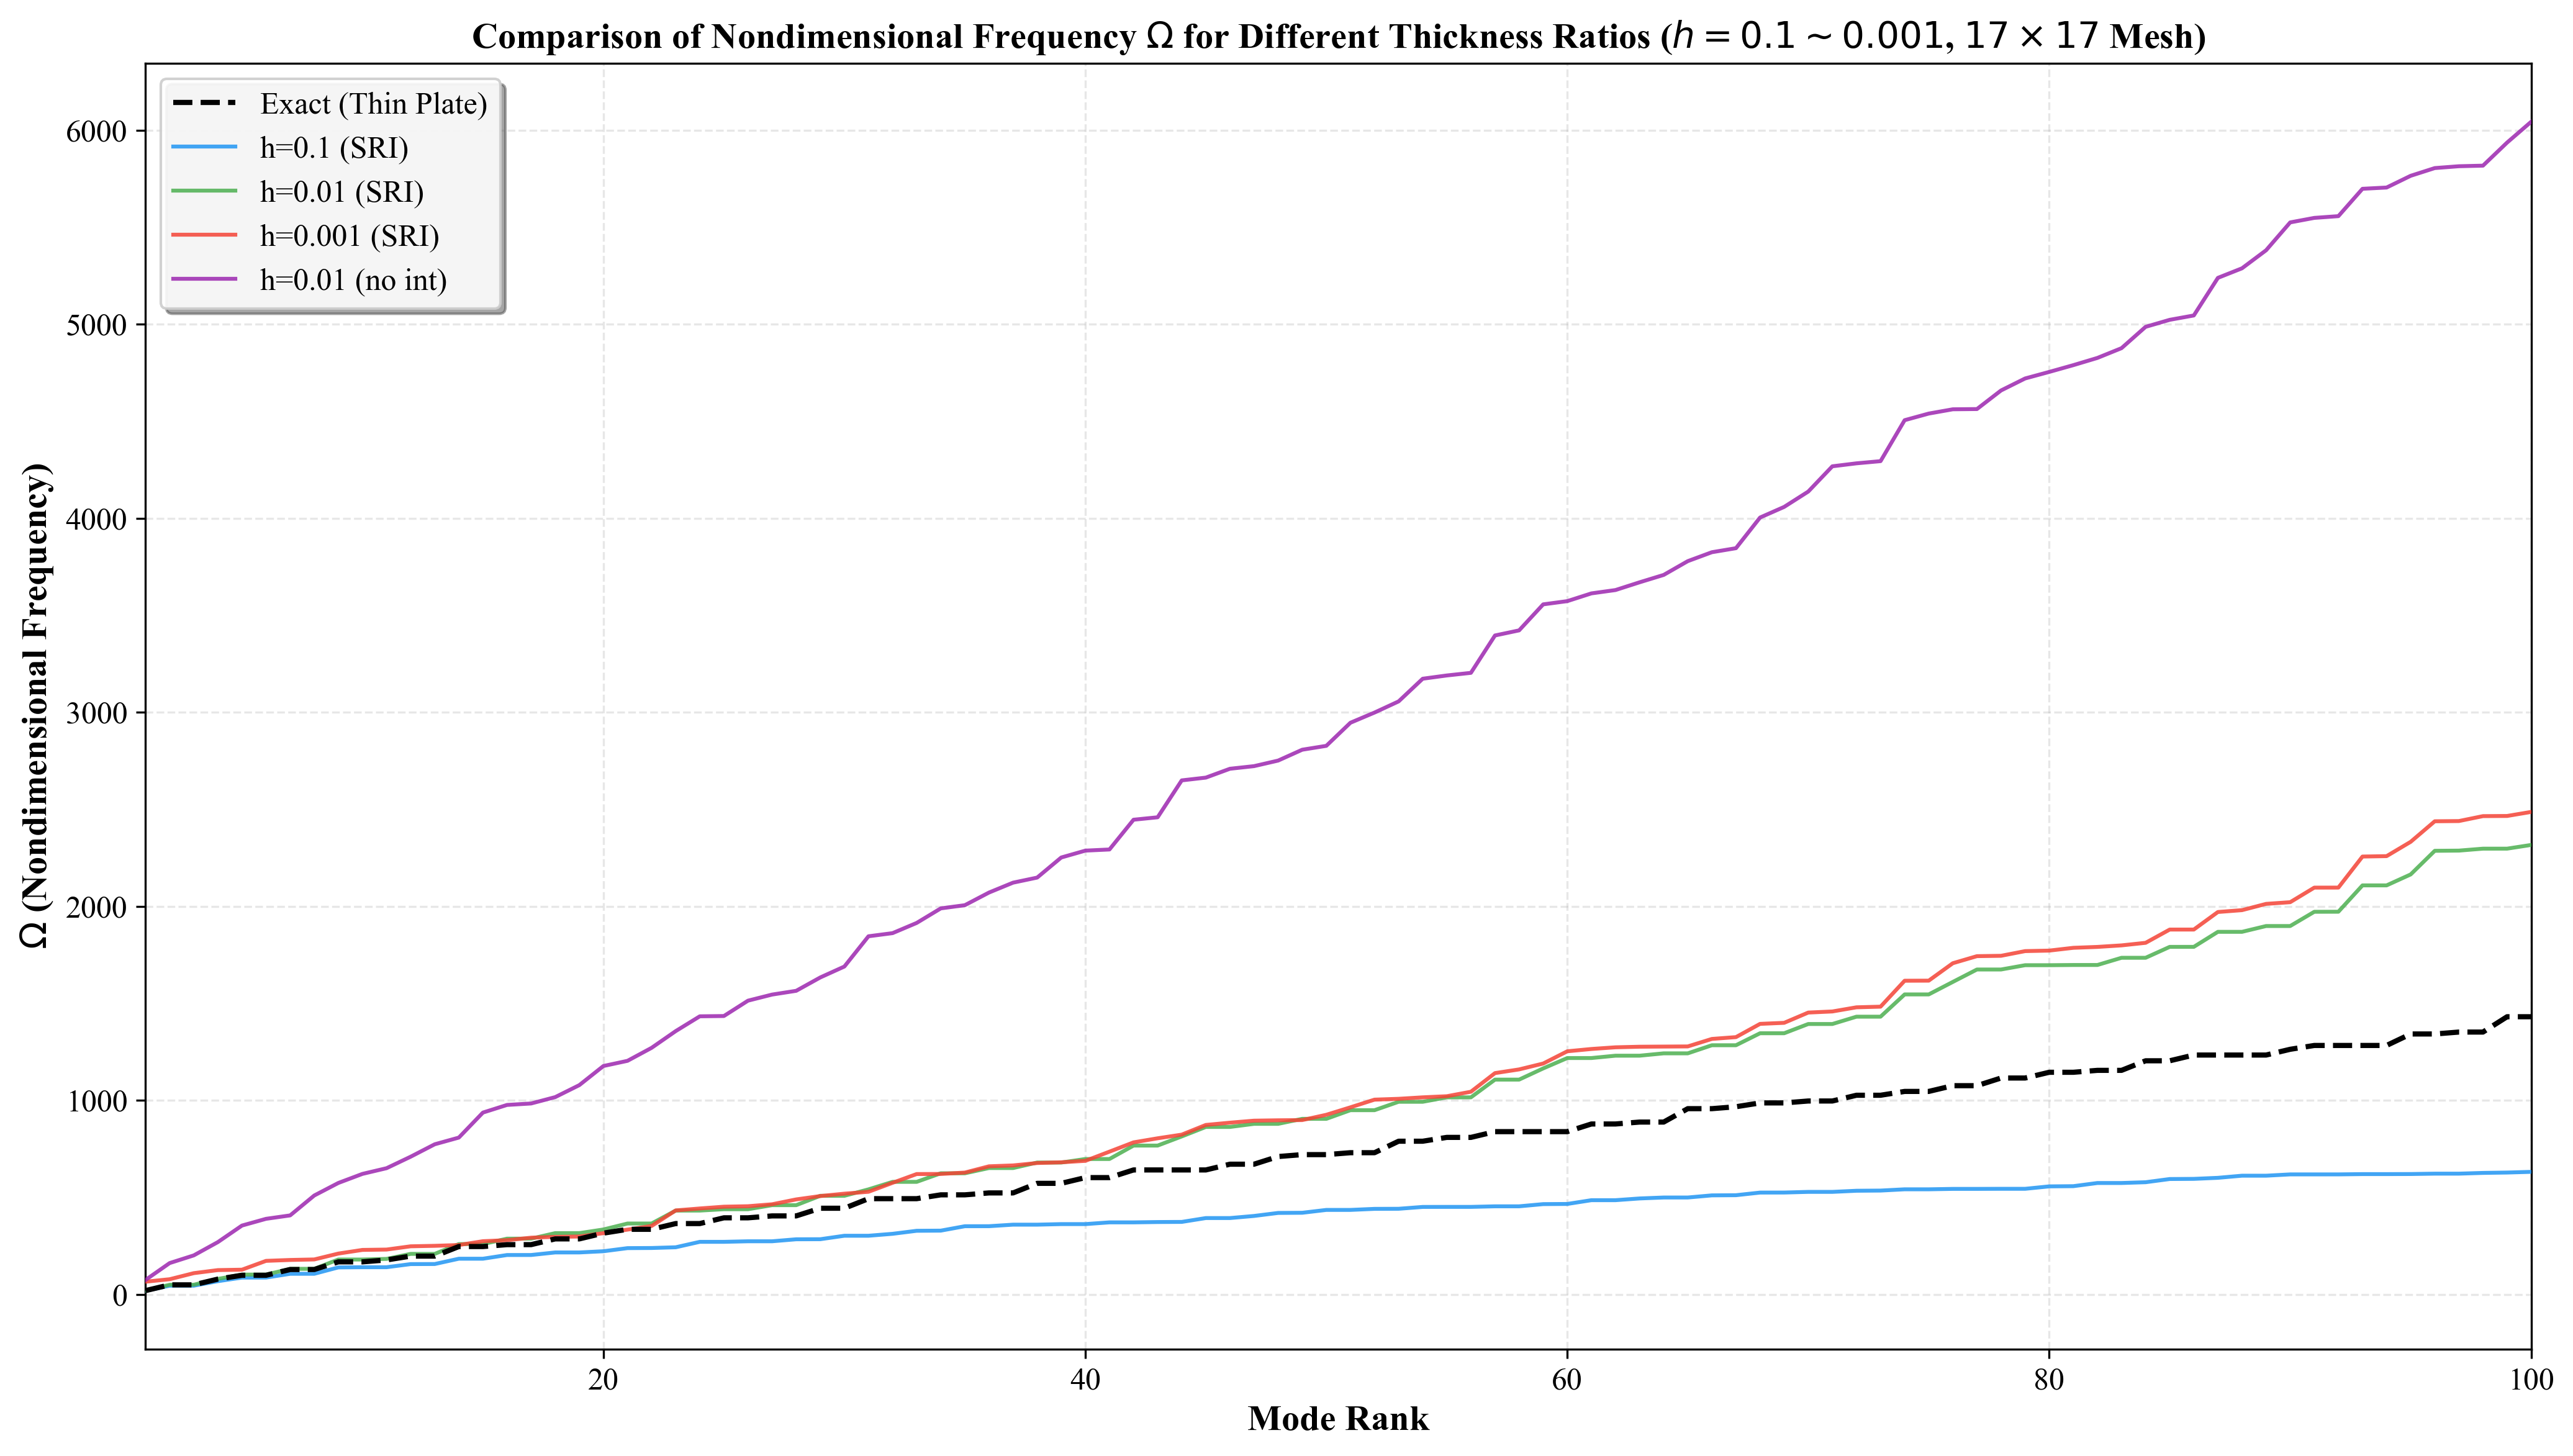
\includegraphics[width=0.9\textwidth]{../../../fig/omega_comparison.png}

        前 100 階模態 $h=0.01$ (SRI) 與精確解幾乎重合

\end{frame}
     % 數據表格 (h=0.1~0.001對齊)

\begin{frame}{科學解密：數值不相容與機器硬體精度溢出}
    \begin{block}{矩陣內部的真實數量級相撞}
        \begin{itemize}
            \item \textbf{實體彎曲剛度劇烈萎縮}：$D^b \propto h^3$。當 $h=0.001, E=10^8$ 時，$D^b \approx \mathbf{0.009157}$。
            \item \textbf{邊界罰剛度恆定巨大}：罰參數 $\alpha = 10^8 \times E = \mathbf{10^{16}}$。
        \end{itemize}
    \end{block}
    \begin{block}{條件數超越硬體精度生死線 (Float64 尾數極限為 $9.0 \times 10^{15}$)}
        \begin{itemize}
            \item \textbf{$h=0.01$ 時}：真實剛度比例 $\frac{\alpha}{D^b} \approx \frac{10^{16}}{9.157} = \mathbf{1.09 \times 10^{15}}$。\\
                  \alert{恰好小於硬體防線}！程式在鋼索邊緣死裡逃生，算出誤差 $-0.21\%$ 的完美解。
            \item \textbf{$h=0.001$ 時}：真實剛度比例飆升至 $\frac{10^{16}}{0.009157} = \mathbf{1.09 \times 10^{18}}$！\\
                  \alert{徹底踩斷硬體防線}！發生數值湮滅，微小的實體剛度資訊被直接抹平截斷，導致全面雪崩。
        \end{itemize}
    \end{block}
\end{frame}     % 機器硬體精度 10^18 數值湮滅解密
\begin{frame}{特徵簡併現象：重根模態子空間旋轉 (MAC $\approx 0.50$)}
    \begin{block}{簡併子空間不變性與隨機旋轉}
        正方形板幾何完全對稱，理論上 $(2,1)$ 與 $(1,2)$ 具有完全相同的重根特徵值（$\Omega=49.348$）。數值特徵值求解器在應對重根時，拋出的兩個向量本質上是理論純模態\textbf{隨機旋轉了約 $45^\circ$ 的線性組合}。
    \end{block}
    \vfill
    \begin{columns}
        \begin{column}{0.48\textwidth}
            \begin{block}{幾何投影定理的精確驗證}
                將混合的對角線棋盤狀波形投影回純理論軸向波形時，其指標值依據投影定理：
                $$\text{MAC} \approx \cos^2(45^\circ) = 0.50$$
            \end{block}
        \end{column}
        \begin{column}{0.48\textwidth}
            \begin{block}{數據退化鏈的有力證實}
                \begin{itemize}
                    \item 在 $h=0.1$ 的厚板微小擾動下，重根 MAC 在 $0.45 \sim 0.49$ 之間擺動。
                    \item 到了 $h=0.01$ 的純淨薄板極限下，對稱性達到極致，第 5、6 階 MAC \textbf{精確收斂至 $0.5000$}。
                \end{itemize}
            \end{block}
        \end{column}
    \end{columns}
\end{frame}% 【全新插入頁】自由振動模態視覺化大圖對比 (包含獨立 Colorbar)
\begin{figure}[htbp]
    \centering
    \begin{subfigure}[b]{0.48\textwidth}
        \centering
        % 導入純淨的正方形九宮格
        
\includegraphics[width=\textwidth]{D:/Joker/Timoshenko/fig/2D_ssss/2d4s_vi_q4_ex/output_grid/17x17_ex_w1_9_grid.png}
        \caption{Navier 級數解析解 (1--9 階)}
    \end{subfigure}
    \hfill
    \begin{subfigure}[b]{0.48\textwidth}
        \centering
        % 導入純淨的正方形九宮格
        
\includegraphics[width=\textwidth]{D:/Joker/Timoshenko/fig/2D_ssss/2d4s_vi_q4_ex/output_grid/17x17_FEM_001_w1_9_grid.png}
        \caption{Q4-SRI h=0.01 數值解 (1--9 階)}
    \end{subfigure}
    
    \vspace{0.3cm} % 留下一點小空隙
    
    \begin{subfigure}[b]{0.48\textwidth}
        \centering
        % 導入純淨的正方形九宮格
        
\includegraphics[width=\textwidth]{D:/Joker/Timoshenko/fig/2D_ssss/2d4s_vi_q4_ex/output_grid/17x17_FEM_001noint_w1_9_grid.png}
        \caption{Q4-SRI h=0.1 數值解 (1--9 階)}
    \end{subfigure}
    
    \hfill
    
    \begin{subfigure}[b]{0.48\textwidth}
        \centering
        % 導入純淨的正方形九宮格
        
\includegraphics[width=\textwidth]{D:/Joker/Timoshenko/fig/2D_ssss/2d4s_vi_q4_ex/17x17_FEM_colorbar.png}
        \caption{Colorbar}
    \end{subfigure}

    \label{fig:modes_1_9_perfect}
\end{figure}     % 重根模態子空間旋轉數學證明

\end{document}